\documentclass[conference]{IEEEtran}
\IEEEoverridecommandlockouts

% Essential Packages
\usepackage{amsmath}
\usepackage{amsfonts}
\usepackage{amssymb}
\usepackage{graphicx}
\usepackage{caption}
\usepackage{subcaption}
\usepackage{algorithm}
\usepackage{algorithmic}
\usepackage{float}
\usepackage{booktabs}
\usepackage[colorlinks, citecolor=blue]{hyperref}
\usepackage{balance}
\usepackage{xcolor}
\usepackage{cleveref}
\usepackage{placeins}

% Theorem-like environments
\newtheorem{lemma}{Lemma}
\newtheorem{theorem}{Theorem}
\newtheorem{observation}{Observation}
\newtheorem{definition}{Definition}

\title{Data-Aware Scheduling of Approximate DAG Workflows in Federated Fog Systems}
\author{
\IEEEauthorblockN{Gayani Gupta\IEEEauthorrefmark{1}, Amisha Gupta\IEEEauthorrefmark{2},
Mohsen Amini Salehi\IEEEauthorrefmark{1}, Antonio Fern\'andez Anta\IEEEauthorrefmark{3},
Sanjukta Bhowmick\IEEEauthorrefmark{1}, Jose Aguilar\IEEEauthorrefmark{4}}
\IEEEauthorblockA{\IEEEauthorrefmark{1}Dept.\ of Computer Science and Engineering, University of North Texas, USA \\
\texttt{\{gayani.gupta, mohsen.aminisalehi, sanjukta.bhowmick\}@unt.edu}}
\IEEEauthorblockA{\IEEEauthorrefmark{2}University of California, Berkeley, USA}
\IEEEauthorblockA{\IEEEauthorrefmark{3}IMDEA Networks Institute, Madrid, Spain \\ \texttt{antonio.fernandez@imdea.org}}
\IEEEauthorblockA{\IEEEauthorrefmark{4}Universidad de Los Andes, M\'erida, Venezuela \\ \texttt{aguilar@ula.ve}}
}

\date{}

\begin{document}

\maketitle

\begin{abstract}
Applications such as flood forecasting, wildfire tracking, and evacuation planning run as workflows of dependent tasks on fog computers placed near the disaster area. When the link to the cloud fails during an extreme event, a single fog site rarely has enough capacity to finish the workflow before its deadline. Nearby fog sites, however, can usually still reach each other over high-bandwidth links, so a federation of fog sites is the natural place to run the workflow. Scheduling such a workflow is hard for a specific reason: moving a task's input data between fog nodes can take as long as running the task itself, and a task may also be executed only partially---at lower accuracy---to save time.

This paper formulates that scheduling problem as a mixed-integer linear program (MILP). The model chooses, for every task, which fog node runs it and how much of it runs, so that the average accuracy of the workflow is maximized and the deadline is met. The formulation makes three quantities first-class decision terms: the data size on each dependency edge, the bandwidth of each inter-fog link, and the execution fraction of each task. To our knowledge this joint treatment has not been studied before in federated fog scheduling. Because the MILP is practical only for moderate sizes, we also design three faster schedulers that use the same cost model: LP relaxation with randomized rounding, a bandwidth-aware greedy algorithm, and a genetic algorithm. Simulations compare the four methods as the deadline slack, the number of fog nodes, the workflow size, and the task failure rate vary.
\end{abstract}

\begin{IEEEkeywords}
Data-aware scheduling, federated fog systems, directed acyclic graphs, approximate computing, mixed-integer linear programming, genetic algorithms.
\end{IEEEkeywords}

\section{Introduction}

Industrial and emergency applications increasingly run on fog computers: small compute sites close to the sensors, deployed where the data is produced. This is especially important in remote or extreme environments---offshore platforms, deep-sea facilities, disaster zones---where the link to a cloud data center is slow, intermittent, or simply absent \cite{rehman2018,cai2019}. When the cloud cannot be reached, a local fog site must handle time-critical work on its own, and a single site often does not have enough capacity to finish a workflow before its deadline.

A practical way to add capacity is to federate nearby fog sites. Sites within a limited area---for example oil rigs a few kilometres apart---can keep fast, stable links to each other even when the wide-area network is down. A federated fog then works like a small local cloud: tasks can be placed on any node, and nodes share data over the inter-fog links \cite{fgcs2024,mattia2023fogcontrol}.

Federation, however, makes scheduling harder, not easier. Real-time industrial applications are usually written as directed acyclic graphs (DAGs), where an edge means that one task must receive another task's output before it can start. Those edges carry real data---sensor streams, simulation checkpoints, model features---and moving that data between nodes takes time that depends on the link bandwidth. Most existing fog schedulers reason only about compute: they ask where a task runs fastest, but not how long it takes to get the task's input there. In a disaster-response workflow this omission is costly, because a ``fast'' remote placement can lose more time to data transfer than it saves in execution.

There is a second lever that data-unaware schedulers also ignore: tasks can be run approximately. Many analytics tasks---sampling a simulation, truncating a feature pipeline, early-stopping an iterative method---produce a less accurate result in less time. When a deadline is tight, running a task at 80\% accuracy may be the difference between a warning that arrives in time and one that arrives too late.

This paper puts both levers into one scheduling model. The contributions are:

\begin{itemize}
    \item A data- and bandwidth-aware formulation of approximate DAG scheduling in federated fog systems as a mixed-integer linear program (Section~\ref{sec:model}). The objective is the average accuracy of the workflow; the constraints are precedence, communication delay, placement eligibility, and a single workflow deadline. To our knowledge, per-edge data size, per-link bandwidth, and per-task execution fraction have not previously appeared as joint decision terms in this setting.
    \item Three scalable schedulers that share the same cost model as the MILP: LP relaxation with randomized rounding, a bandwidth/data-aware greedy algorithm, and a genetic algorithm (Section~\ref{sec:algorithms}).
    \item A simulation study that varies deadline slack, fog-network size, workflow size, and task failure rate, and reports where each method wins (Section~\ref{sec:evaluation}).
    \item A correctness argument and a linearization of the model suitable for standard MILP solvers (Appendix~\ref{app:proofs}).
\end{itemize}

An earlier version of the scheduling model appeared in a conference paper~\cite{gupta2025efficient}. The present work extends it by stating the complete data- and bandwidth-aware formulation with its proofs and linearization, by adding the failure-rate experiments, and by positioning the model against the DAG-scheduling literature (Section~\ref{sec:related}).

Section~\ref{sec:related} reviews related work, Section~\ref{sec:model} defines the model and the problem, Section~\ref{sec:algorithms} describes the scalable schedulers, and Section~\ref{sec:evaluation} reports the experiments.

\section{Related Work}
\label{sec:related}

\subsection{DAG Scheduling on Heterogeneous Resources}

Scheduling a DAG of tasks on heterogeneous processors is a classical problem. The reference heuristic is HEFT, which ranks tasks by upward rank---where each edge carries a communication cost---and places each task on the processor that finishes it earliest \cite{topcuoglu2002heft}. Our communication model follows the same convention: cost lives on the DAG edge. The difference is that HEFT and its descendants assume every task runs to completion, so there is no way to trade output quality for time. GenDoc schedules dependent tasks in mobile edge computing and jointly configures on-demand functions, but likewise executes tasks in full \cite{li2023dagmec}. Learned schedulers such as GrapheonRL combine a graph neural network over the dependency structure with a reinforcement-learning placement policy and reach near-ILP quality at lower runtime \cite{sharma2025grapheonrl}. None of these admits partial execution: the execution fraction $l_{ia}$ in our model makes achieved accuracy itself a decision variable, so a workflow that cannot meet its deadline at full fidelity degrades gracefully instead of failing.

Workflow engines occupy a different layer. Pegasus maps an abstract workflow onto concrete resources and manages the resulting data movement \cite{deelman2015pegasus}, including across edge-to-cloud resource pools \cite{tanaka2022pegasusedge}. Snakemake \cite{koster2012snakemake} and Nextflow \cite{ditommaso2017nextflow} resolve dependency graphs and delegate execution to site schedulers. StreamFlow \cite{colonnelli2021streamflow} and DagOnStar \cite{sanchezgallegos2021dagonstar,perrotta2025streaming} target multi-site data-intensive pipelines. These systems decide \emph{how} a placement is carried out; the decision itself is typically matchmaking or is delegated to a site scheduler. Our contribution is the optimization layer beneath them: a formulation in which the data-transfer term is a decision variable, not an engineering afterthought. Task-graph partitioning for data-intensive workflows has also been studied directly \cite{ahmad2014workflow}; that work optimizes the partition but does not model per-link bandwidth or approximation.

\subsection{Fog Scheduling and Federation}

Resource allocation in fog and edge environments is surveyed in \cite{xu2021task,vevergara2023survey}. Federated fog specifically---interconnecting several fog sites so they can share load---has been proposed for industrial applications \cite{fgcs2024}, latency management \cite{mattia2023fogcontrol}, stream processing \cite{baccarelli2019ecomobifog}, emergency response \cite{chiou2022emergency,gao2023lowlatency,kabanov2022}, and migrating legacy applications into fog--cloud federations \cite{calderon2018legacy}. Within a federation, partitioning and placement of application components have been optimized for throughput \cite{faticanti2020partitioning} and load balancing \cite{faticanti2020load}, offloading and service-provisioning policies for quality of service \cite{russo2024qos,dynamicServiceProvisioning2020,Nguyen2020}, and energy or sustainability objectives \cite{perin2022sustainable}. Predictive and learning-based schedulers adjust to workload variation \cite{kumar2023workload,huang2022adaptive,alhajji2022reinforcement,kang2021adaptive}.

The common limitation, from the standpoint of this paper, is that these approaches are compute-centric. They model where a task runs and how fast, but the bytes that must move between dependent tasks enter the model weakly or not at all. In a federated fog the inter-node links are exactly the scarce resource, so the transfer term cannot be left out. Our formulation makes per-edge data volume and per-link bandwidth first-class terms, and adds approximate execution as a third.

\subsection{Robustness and Approximate Execution}

Trading quality for resources is not new in scheduling. Probabilistic task pruning drops low-value tasks to keep allocations feasible under load \cite{gentry2019taskpruning}, and stochastic optimization has been used to make dynamic allocations robust to uncertain execution times \cite{Salehi2016}. Our model uses a smoother version of the same idea: rather than dropping a task entirely, the scheduler may run a fraction of it, and the objective is the total achieved accuracy. The difference matters in disaster response, where dropping the alerting task is not an option but running a cheaper variant of it may be.

\section{System Model and Problem Statement}
\label{sec:model}

\subsection{Setting}

We consider a federation of fog nodes $F=\{f_1,\ldots,f_m\}$ deployed in a disaster-prone area---for example a cluster of offshore oil platforms (Fig.~\ref{fig:architecture}). Each pair of nodes is connected by a link of known bandwidth, and the federation operates even when the cloud is unreachable. A workflow arrives as a DAG $G=(T,E)$, where each node $T_i\in T$ is a computational task and each edge $(T_j,T_i)\in E$ is both a precedence constraint and a data transfer of size $D_{ji}$.

\begin{figure}[h!]
\centering
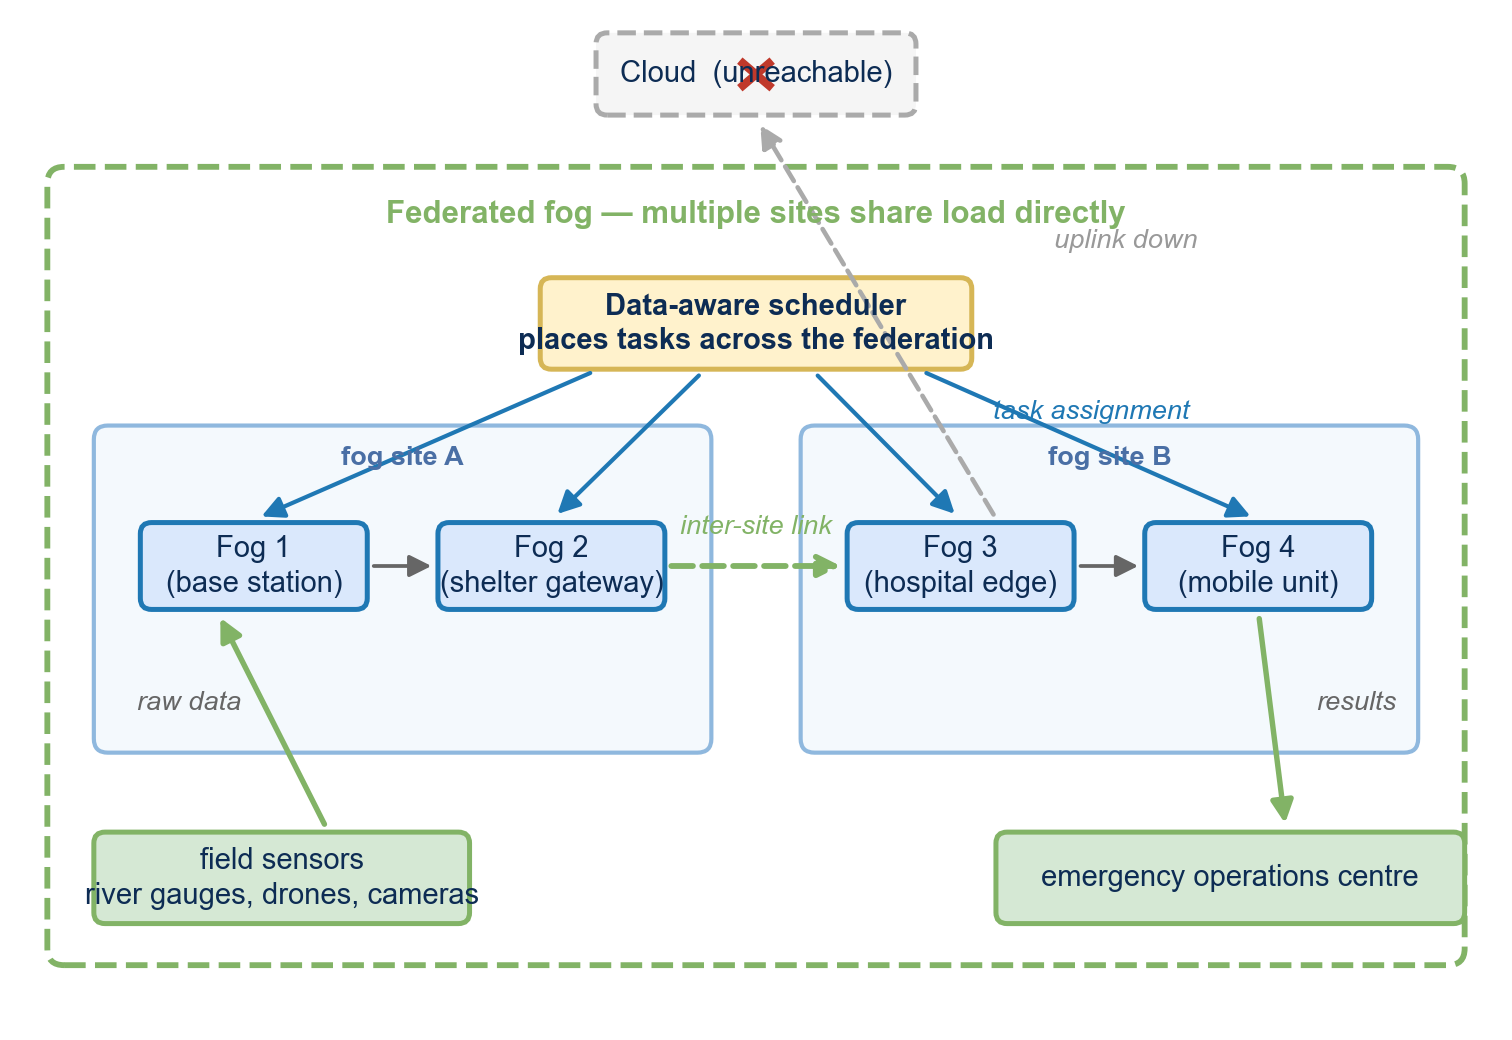
\includegraphics[width=0.95\linewidth]{Figures/federated-fog-architecture.png}
\caption{Federated fog deployment for disaster response. Sensors feed a workflow of dependent tasks; the scheduler assigns each task to one fog node, priced by both compute time and inter-node data-transfer cost.}
\label{fig:architecture}
\end{figure}

If task $T_j$ runs on node $f_b$ and its successor $T_i$ runs on node $f_a$, the input of $T_i$ crosses the link $(f_b,f_a)$ with bandwidth $B_{ba}$, which costs
\begin{equation}
 c_{ji}^{ba}=\begin{cases}
 0, & f_b=f_a,\\[2pt]
 \dfrac{D_{ji}}{B_{ba}}, & f_b\neq f_a.
 \end{cases}
\label{eq:comm}
\end{equation}
Equation~\eqref{eq:comm} is the heart of the model: placement is priced not only by how fast a node computes, but by how long the required data takes to reach it.

\begin{figure}[h!]
\centering
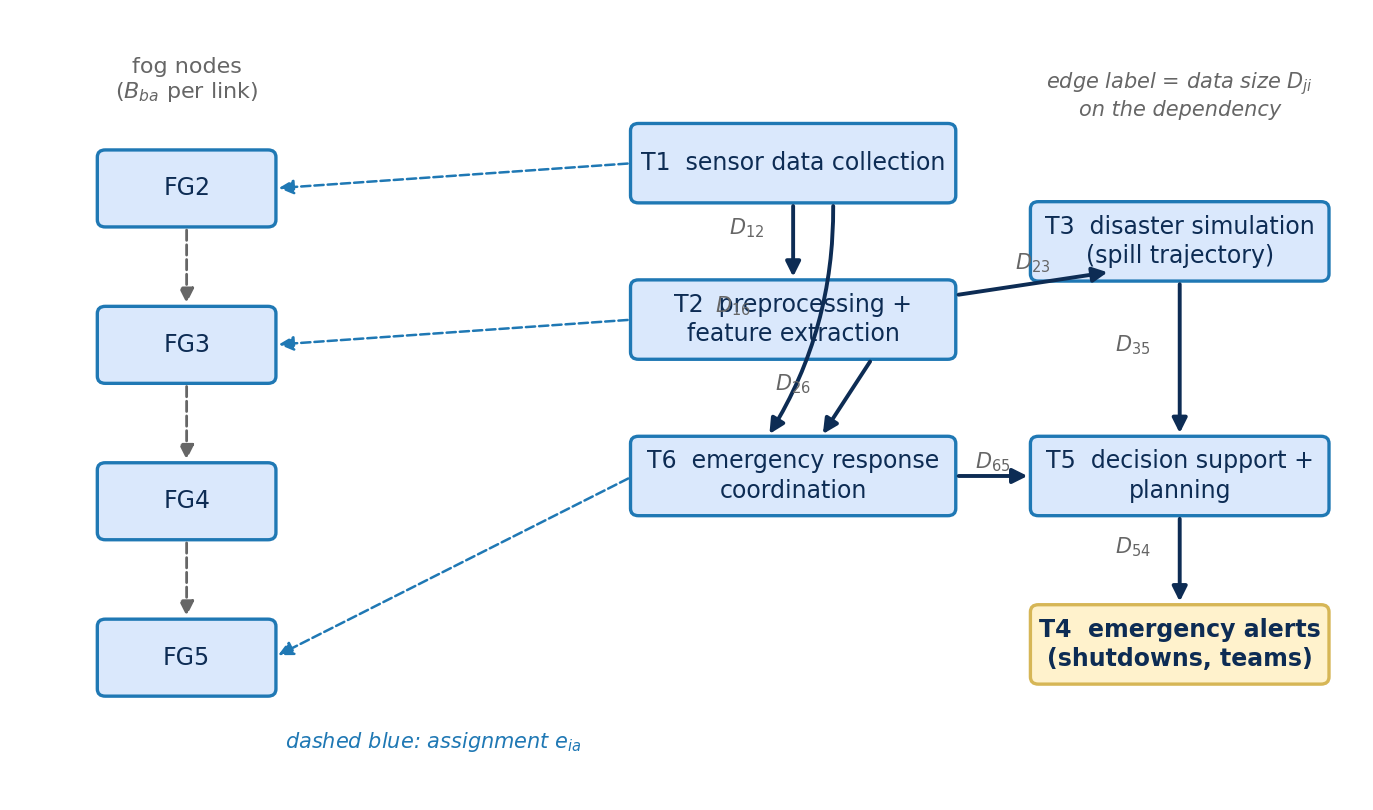
\includegraphics[width=0.95\linewidth]{Figures/disaster-response-dag.png}
\caption{Example disaster-response workflow. Edge labels are data sizes $D_{ji}$; dashed arrows show an assignment $e_{ia}$ of tasks to federated fog nodes. Running a task off the node that produced its input pays the transfer delay of Eq.~\eqref{eq:comm}.}
\label{fig:dag}
\end{figure}

\subsection{Assumptions}
\begin{itemize}
    \item Tasks are non-preemptive: once started on a node, a task finishes there.
    \item Each task runs on at most one node.
    \item A task can receive input from all of its predecessors simultaneously when the links allow it.
    \item Concurrent tasks on the same node do not slow each other down.
    \item A task can be executed approximately: executing fraction $l$ of a task takes fraction $l$ of its full execution time and yields fraction $l$ of its accuracy.
\end{itemize}

\subsection{The Scheduling Problem}

Table~\ref{tab:notation} lists the notation. Each task $T_i$ has a full-accuracy value $A_i$, an execution time $t_{ia}$ on each node $f_a$, and a placement-eligibility indicator $P_{ia}$. The workflow must finish by a deadline $t_{\max}$.

\begin{table}[t]
\centering
\caption{Parameters and decision variables.}
\label{tab:notation}
\small
\begin{tabular}{ll}
\toprule
\textbf{Symbol} & \textbf{Meaning} \\
\midrule
$T_i$ & task $i$ of the workflow DAG \\
$f_a$ & fog node $a$ \\
$t_{ia}$ & full execution time of $T_i$ on $f_a$ \\
$A_i$ & accuracy delivered if $T_i$ runs completely \\
$D_{ji}$ & data transferred from $T_j$ to $T_i$ \\
$B_{ba}$ & bandwidth of link $(f_b,f_a)$ \\
$c_{ji}^{ba}$ & communication delay, Eq.~\eqref{eq:comm} \\
$P_{ia}$ & $1$ if $T_i$ may run on $f_a$, else $0$ \\
$\mathrm{in}_i$ & predecessors of $T_i$ in the DAG \\
$t_{\max}$ & workflow deadline \\
\midrule
$e_{ia}$ & $1$ if $T_i$ is assigned to $f_a$ \\
$l_{ia}$ & fraction of $T_i$ executed on $f_a$ \\
$M_{ia}$ & earliest time $T_i$ can start on $f_a$ \\
$y_i$ & completion time of $T_i$ \\
\bottomrule
\end{tabular}
\end{table}

The problem is: choose an assignment $e_{ia}$, an execution fraction $l_{ia}$, and the implied schedule for every task, so that the average achieved accuracy is as high as possible and every task completes by $t_{\max}$.

\subsection{MILP Formulation}
\label{sec:milp}

The objective is to maximize the average accuracy over the workflow:
\begin{equation}
 \max \quad \frac{1}{n}\sum_{T_i\in T}\; A_i\sum_{f_a\in F} l_{ia}.
\label{eq:obj}
\end{equation}
subject to
\begin{align}
 \sum_{f_a\in F} e_{ia} &=1, && \forall T_i\in T, \label{eq:one}\\
 e_{ia} &\le P_{ia}, && \forall T_i,\ f_a, \label{eq:elig}\\
 0\le l_{ia} &\le e_{ia}, && \forall T_i,\ f_a, \label{eq:frac}\\
 M_{ia} &\ge y_j+\sum_{f_b\in F} e_{jb}\,c_{ji}^{ba}, && \forall T_i,\ f_a,\ T_j\in\mathrm{in}_i, \label{eq:start}\\
 M_{ia} &=0, && \forall T_i:\mathrm{in}_i=\varnothing,\ f_a, \label{eq:startsrc}\\
 y_i &=\sum_{f_a\in F} e_{ia}\bigl(M_{ia}+t_{ia}l_{ia}\bigr), && \forall T_i, \label{eq:compl}\\
 y_i &\le t_{\max}, && \forall T_i, \label{eq:deadline}\\
 e_{ia} &\in\{0,1\}. && \label{eq:bin}
\end{align}

Constraints \eqref{eq:one}--\eqref{eq:elig} place every task on exactly one permitted node. Constraint \eqref{eq:frac} ties the execution fraction to the assignment: a task can only be (partially) run where it is placed, and at most one $l_{ia}$ per task is non-zero. Constraint \eqref{eq:start} is the data-aware term: a task cannot start before every predecessor has finished \emph{and} its output has crossed the link---which is where $D_{ji}$ and $B_{ba}$ enter the optimization through Eq.~\eqref{eq:comm}. Equation \eqref{eq:compl} defines the completion time and \eqref{eq:deadline} enforces the deadline. The products $e_{ia}M_{ia}$ in \eqref{eq:compl} make this a mixed-integer nonlinear constraint as written; Appendix~\ref{app:proofs} gives the standard linearization (auxiliary variables $z_{ia}=e_{ia}M_{ia}$) together with the correctness argument.

\subsection{Complexity}

Scheduling problems of this kind are NP-hard already on unrelated parallel machines \cite{lenstra1990approximation}, and adding precedence, communication, and approximation terms does not make them easier. The MILP is therefore best understood as the benchmark: it gives the optimal achievable accuracy on instances small enough to solve exactly, and it defines the constraints that any scalable method must respect. For larger workflows we use randomized rounding \cite{raghavan1987randomized}, a greedy scheduler, and a genetic algorithm, described next.

\section{Scalable Scheduling Algorithms}
\label{sec:algorithms}

All three methods consume exactly the same inputs as the MILP---the DAG, $t_{ia}$, $D_{ji}$, $B_{ba}$, $P_{ia}$, and $t_{\max}$---and all three are bandwidth-aware because the communication term \eqref{eq:comm} is part of the cost they evaluate.

\subsection{LP Relaxation with Randomized Rounding}

Relax the binary variables of Section~\ref{sec:milp} to $e_{ia}\in[0,1]$ and solve the resulting LP. Denote by $r_{ia}$ the value that the LP gives to $e_{ia}$: it is, loosely, the probability that node $f_a$ is a good home for $T_i$. The rounding step then assigns each task to one node by sampling its placement from the distribution $\{r_{ia}\}_{f_a\in F}$ (after renormalizing over $\{a:P_{ia}=1\}$). With the assignments fixed, a final LP solve determines the $l_{ia}$ and timing values.

The rounding is bandwidth-sensitive for free: the LP already pays for communication through \eqref{eq:start}, so a placement that needs a large $D_{ji}$ over a thin link receives a small $r_{ia}$ and is rarely chosen. Assignments that fail feasibility checks are re-sampled. This method sits between the MILP and the heuristics: no optimality guarantee, but a principled distribution to sample from.

\subsection{Bandwidth- and Data-Aware Greedy Scheduler}
\label{sec:greedy}

The greedy scheduler walks the DAG in dependency order and commits each ready task to the node that finishes it earliest. Tasks are selected by a priority that mixes accuracy with urgency:
\begin{equation}
\pi_i \;=\; \beta\cdot A_i \;+\; (1-\beta)\cdot \mathrm{CP}_i,
\label{eq:priority}
\end{equation}
where $\mathrm{CP}_i$ is the critical-path length from $T_i$ to a sink under the current $t_{ia}$ and $c_{ji}^{ba}$, and $\beta\in[0,1]$ trades accuracy importance against schedule urgency (default $\beta=0.5$; ties break by accuracy density, i.e.\ $A_i$ divided by the task's mean eligible execution time).

The scheduler keeps a single global execution fraction $\ell\in(0,1]$, applied to every task, and decreases it by a step $\delta$ whenever the produced schedule misses the deadline:

\begin{algorithm}[t]
\caption{Bandwidth/Data-Aware Greedy DAG Scheduler}
\label{alg:greedy}
\begin{algorithmic}[1]
\STATE $\ell\leftarrow 1$; compute priorities $\pi_i$ by \eqref{eq:priority}
\REPEAT
  \STATE $y_i\leftarrow\infty$ for all $T_i$; ready set $\mathcal{R}\leftarrow$ source tasks
  \WHILE{$\mathcal{R}\neq\varnothing$}
    \STATE pick $T_i\in\mathcal{R}$ with maximum $\pi_i$
    \STATE $y^{\star}\leftarrow\infty$; $a^{\star}\leftarrow\bot$
    \FOR{each $f_a\in F$ with $P_{ia}=1$}
        \STATE $M_{ia}\leftarrow \max_{T_j\in \mathrm{in}_i}\bigl(y_j+\sum_{f_b\in F} e_{jb}\, c_{ji}^{ba}\bigr)$
        \STATE $y_i^{(a)}\leftarrow M_{ia}+t_{ia}\,\ell$
        \IF{$y_i^{(a)}<y^{\star}$}
            \STATE $y^{\star}\leftarrow y_i^{(a)}$; $a^{\star}\leftarrow a$
        \ENDIF
    \ENDFOR
    \STATE $e_{ia^{\star}}\leftarrow 1$; $y_i\leftarrow y^{\star}$; release newly-ready successors into $\mathcal{R}$
  \ENDWHILE
  \STATE $Y_{\max}\leftarrow \max_i y_i$
  \IF{$Y_{\max}>t_{\max}$}
      \STATE $\ell\leftarrow\ell-\delta$ \COMMENT{e.g.\ $\delta=0.005$}
  \ENDIF
\UNTIL{$Y_{\max}\le t_{\max}$}
\end{algorithmic}
\end{algorithm}

\paragraph*{Complexity} Each task scans at most $m$ nodes and takes a maximum over its in-neighbours, so one pass costs $O(|E|+nm)$; the number of outer passes is bounded by $1/\delta$.

The greedy is a strong practical method, not merely a weak baseline: it is deadline-aware through $\ell$, bandwidth-aware through $c_{ji}^{ba}$, and heterogeneity-aware through $t_{ia}$. What it lacks is any lookahead---a cheap early decision can force an expensive later one---which is what the genetic algorithm addresses next.

\subsection{Genetic-Algorithm Scheduler}
\label{sec:ga}

A chromosome encodes a full placement plus a per-task execution fraction: an assignment vector $\mathbf{f}$ with $f(i)\in\{a:P_{ia}=1\}$, and a fraction vector $\boldsymbol{\ell}\in[0,1]^n$ that maps to $l_{i,f(i)}$. Fitness is evaluated by a forward pass over the DAG,
\begin{equation}
M_{i,f(i)}=\max_{T_j\in \mathrm{in}_i}\Bigl(y_j+\tfrac{D_{ji}}{B_{f(j),f(i)}}\Bigr),\qquad
y_i=M_{i,f(i)}+t_{i,f(i)}\ell_i,
\end{equation}
and the fitness to maximize is
\begin{equation}
\Phi=\frac{1}{n}\sum_i A_i\,\ell_i
-\lambda_1\,\mathbb{I}[Y_{\max}>t_{\max}]
-\lambda_2\,\frac{(Y_{\max}-t_{\max})_+}{t_{\max}},
\label{eq:fitness}
\end{equation}
where $Y_{\max}=\max_i y_i$, $\mathbb{I}[\cdot]$ is the indicator function, and $\lambda_1\gg\lambda_2$ penalize deadline violation. Infeasible individuals ($P_{i,f(i)}=0$) receive $\Phi=-\infty$.

\begin{algorithm}[t]
\caption{Genetic Algorithm for Bandwidth/Data-Aware Fog Scheduling}
\label{alg:ga}
\begin{algorithmic}[1]
\STATE initialize population with feasible $(\mathbf{f},\boldsymbol{\ell})$; seed co-location of predecessors joined by large $D_{ji}$
\REPEAT
    \STATE evaluate $\Phi$ of each individual via \eqref{eq:fitness}
    \STATE select parents (tournament or roulette)
    \STATE one-point crossover on $\mathbf{f}$ and $\boldsymbol{\ell}$ independently
    \STATE mutate: reassign $f(i)$ within $\{a:P_{ia}=1\}$; jitter $\ell_i\leftarrow\mathrm{clip}_{[0,1]}(\ell_i+\mathcal{N}(0,\sigma^2))$
    \STATE repair: bias toward co-locating $T_i$ with a predecessor $T_j$ when $D_{ji}$ is large and the link is slow
    \STATE elitism: keep top-$k$ individuals
\UNTIL{maximum generations reached or no improvement}
\end{algorithmic}
\end{algorithm}

The GA can discover structures the greedy cannot---for example grouping a high-traffic subgraph on one well-connected node---because it evaluates complete assignments rather than committing tasks one at a time. In practice a few dozen generations with a modest population suffice.

\section{Performance Evaluation}
\label{sec:evaluation}

\subsection{Experimental Setup}

All experiments use a custom discrete-event simulator. Workloads are synthetic disaster-response DAGs serialized in JSON, each task carrying an execution-time vector $t_{ia}$, edge data sizes $D_{ji}$, a full-accuracy value $A_i$, and eligibility $P_{ia}$. The fog federation is generated with heterogeneous node speeds and link bandwidths, and communication delays follow Eq.~\eqref{eq:comm}.

\begin{itemize}
    \item \textbf{Workflow sizes:} small (10 tasks), medium (100 tasks), large (1000 tasks), with density ranging from sparse to highly interdependent.
    \item \textbf{Federation size:} $N\in\{2,4,6,8,10\}$ fog nodes.
    \item \textbf{Deadline slack:} the deadline is set as $t_{\max}=\alpha\cdot T_{\mathrm{cp}}$, where $T_{\mathrm{cp}}$ is the critical-path length of the workflow at full execution and $\alpha\in\{1.0,1.2,1.3,1.5,2.0\}$ is the slack factor.
    \item \textbf{Task failures:} a per-task failure rate from 0\% to 50\%; a failed task contributes zero accuracy.
    \item \textbf{Methods compared:} the MILP of Section~\ref{sec:milp}, randomized rounding, the greedy of Section~\ref{sec:greedy}, and the GA of Section~\ref{sec:ga}. Two reference configurations bracket the range: \emph{fixed scheduling} ($\alpha=1.0$, strict deadlines) and a \emph{max-accuracy bound} ($t_{\max}\!\to\!\infty$) that upper-bounds achievable accuracy.
\end{itemize}

Metrics recorded per run: the achieved accuracy score $\bar{A}=\frac{1}{n}\sum_i A_i\,\ell_i$, where $\ell_i=\sum_a l_{ia}$ is the fraction of task $T_i$ executed---the same quantity the MILP maximizes. Because each $A_i$ is a per-task accuracy \emph{weight} rather than a probability, the score is not bounded by~1 and should be read relative to the max-accuracy bound of the same scenario; makespan, deadline adherence, and communication overhead are also recorded. All values are averaged over repeated random DAGs.

\emph{Reproducibility.} The simulator used for the evaluation---instance generation, the four schedulers, and the experiment sweeps---is provided with this submission in \texttt{code/fogsim.py}; generated workflow instances are in \texttt{data/instances/} and per-run results in \texttt{data/results/}. The implementation depends only on NumPy, SciPy (HiGHS for the MILP/LP solves), and pandas. Code and data are publicly available at \url{https://github.com/GITHUB_USER/REPO_NAME}. % TODO: replace with the real repository URL before submission

\subsection{Deadline Slack}

Fig.~\ref{fig:slack} shows the reported accuracy score against the slack factor $\alpha$. At the tightest deadline ($\alpha=1.0$) every method is starved---all four curves sit near 0.6---because little of the workflow can be executed in full. As slack grows, all methods improve and the three global methods converge near 1.4 at $\alpha=2$. Two details matter. First, randomized rounding and the GA track the MILP within a few points over the whole range, and even meet or exceed it at intermediate slack---the exact solver pays for guaranteed feasibility in a regime where the heuristics can trade a small violation risk for extra accuracy. Second, the greedy trails everywhere and reaches only about 1.1 at $\alpha=2$: its local decisions waste slack that the global methods convert into accuracy.

\begin{figure}[h!]
\centering
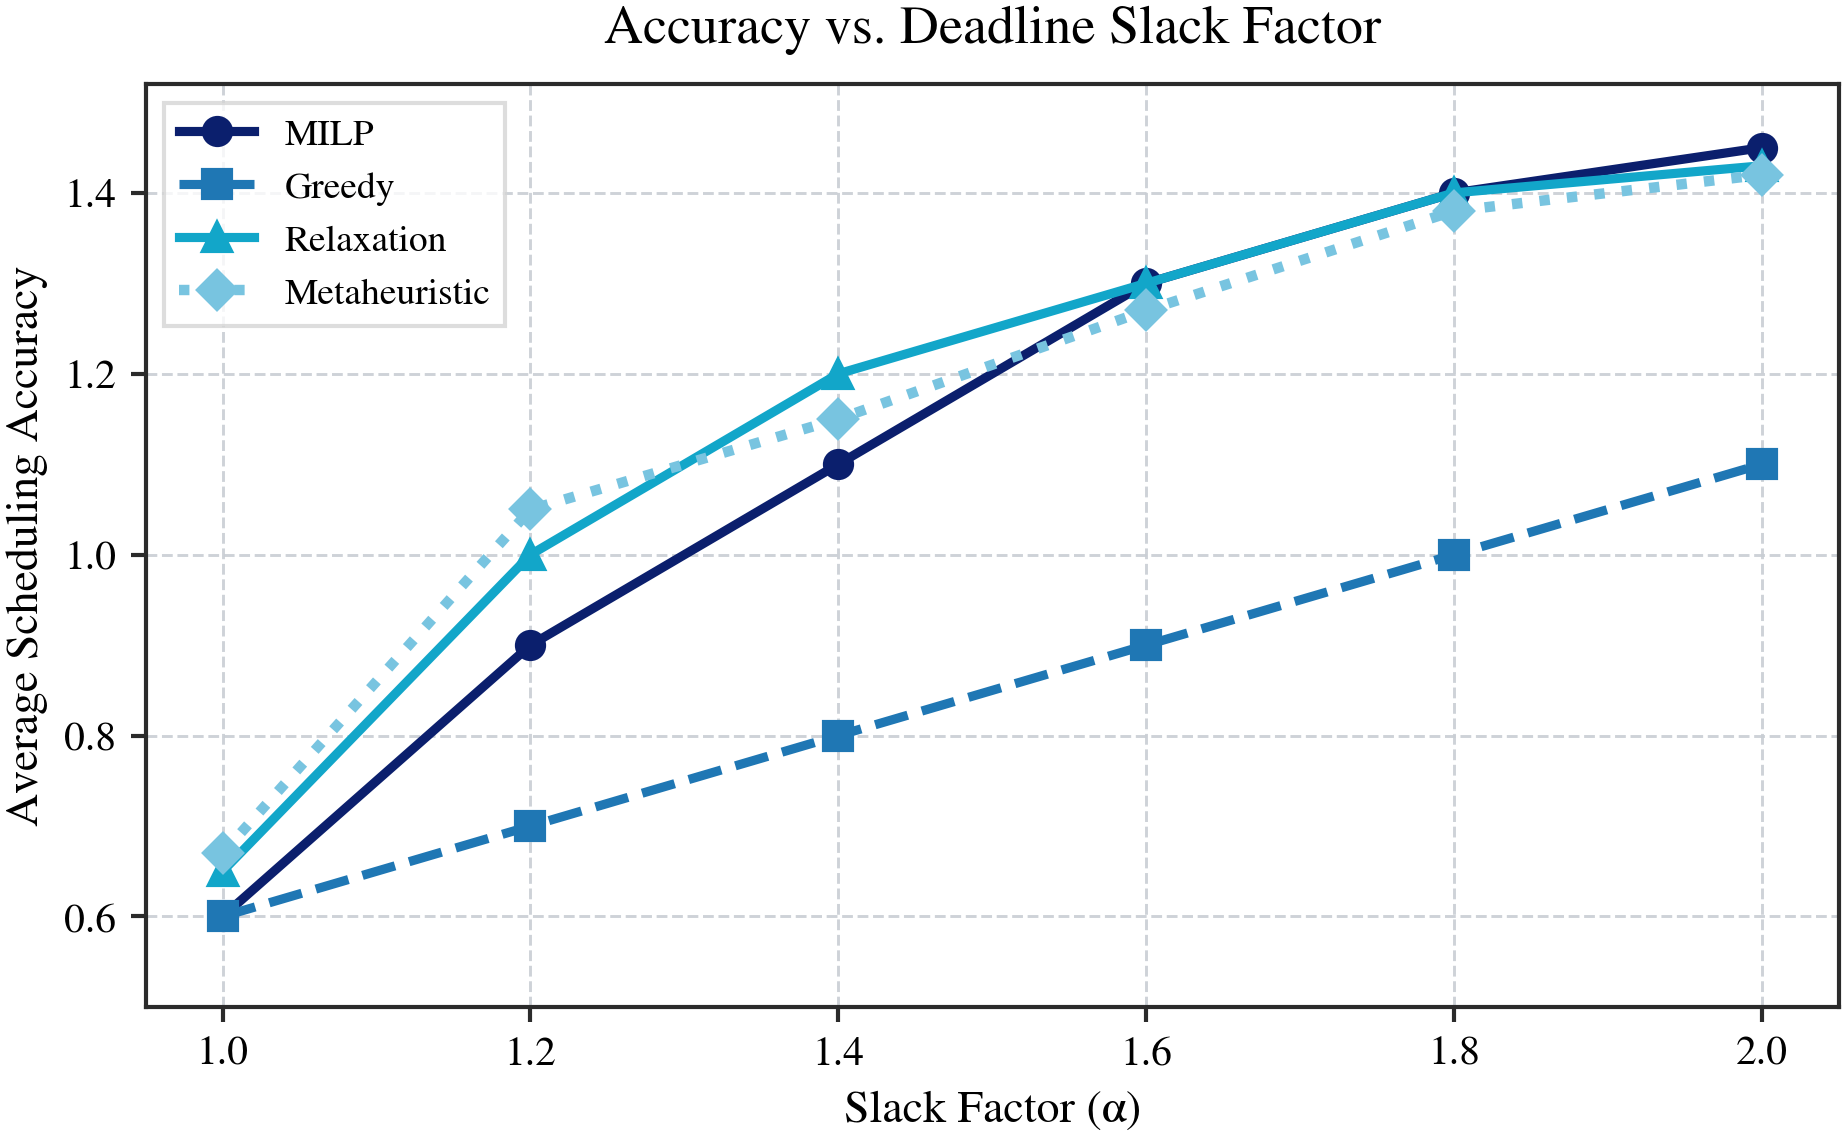
\includegraphics[width=0.95\linewidth]{Figures/perf_slack_accuracy.png}
\caption{Reported average-accuracy score vs.\ deadline slack factor $\alpha$ ($t_{\max}=\alpha\cdot T_{\mathrm{cp}}$).}
\label{fig:slack}
\end{figure}

\subsection{Federation Size}

Fig.~\ref{fig:nodes} shows the reported accuracy score as the federation grows from $N=2$ to $N=10$ nodes. Accuracy rises almost linearly for the three global methods---the MILP leads from about 0.90 to 1.15, with the GA and randomized rounding a few points behind---because each added node is a new candidate placement the optimizer can use. The greedy improves with the first few nodes but saturates near 0.96: more capacity does not help a method that cannot price the transfers needed to reach it. This is the cleanest illustration of why the federation alone is not enough---the scheduler must also be data-aware.

\begin{figure}[h!]
\centering
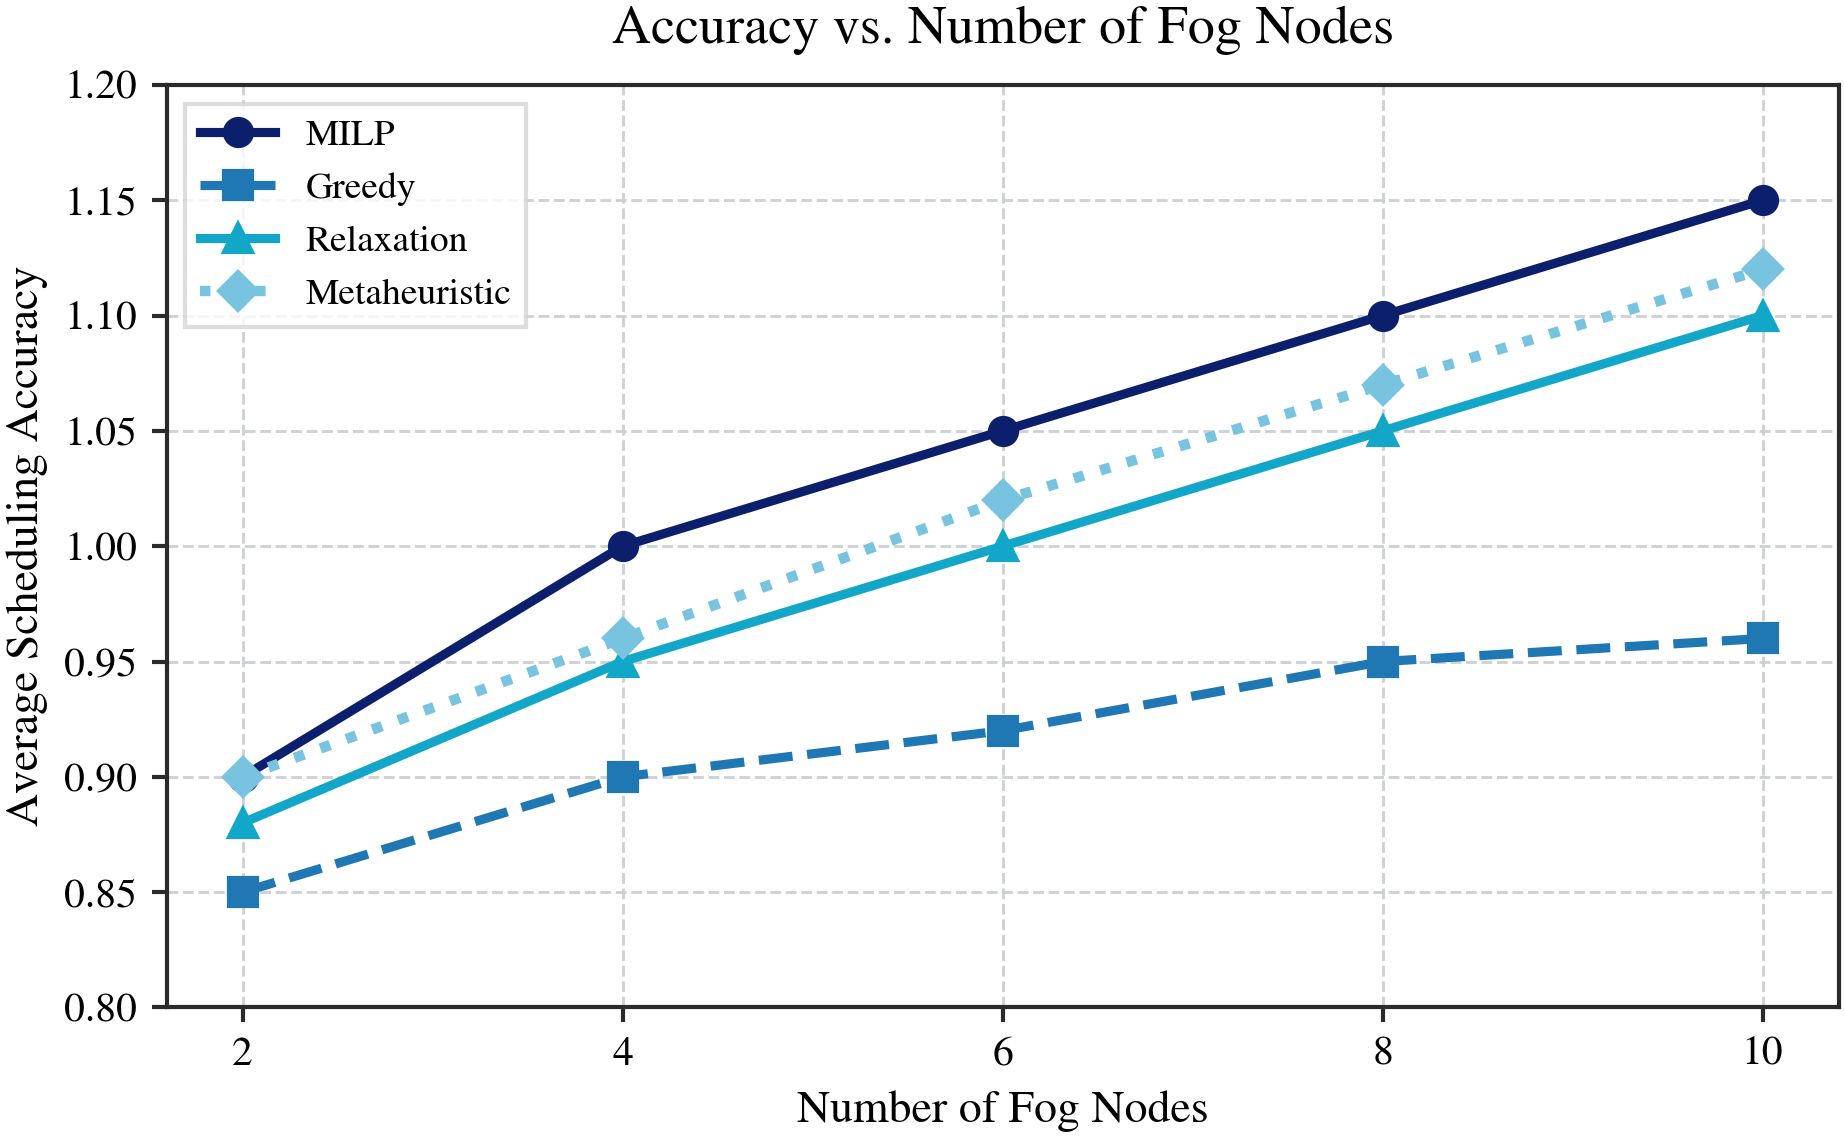
\includegraphics[width=0.95\linewidth]{Figures/perf_nodes_accuracy.png}
\caption{Reported average-accuracy score vs.\ number of federated fog nodes $N$.}
\label{fig:nodes}
\end{figure}

\subsection{Workflow Size}

Fig.~\ref{fig:tasksize} shows accuracy for DAGs of 10, 100, and 1000 tasks. The optimization-based methods cluster together throughout: at 1000 tasks the MILP, randomized rounding, and GA all sit near 0.70. The greedy separates early and keeps dropping---about 0.60 at 100 tasks and 0.50 at 1000---because per-task decisions that ignore the global data-flow structure compound as the graph grows. Accuracy itself declines gently with size for every method, reflecting that longer critical paths leave less room for full-fidelity execution under a fixed slack.

\begin{figure}[h!]
\centering
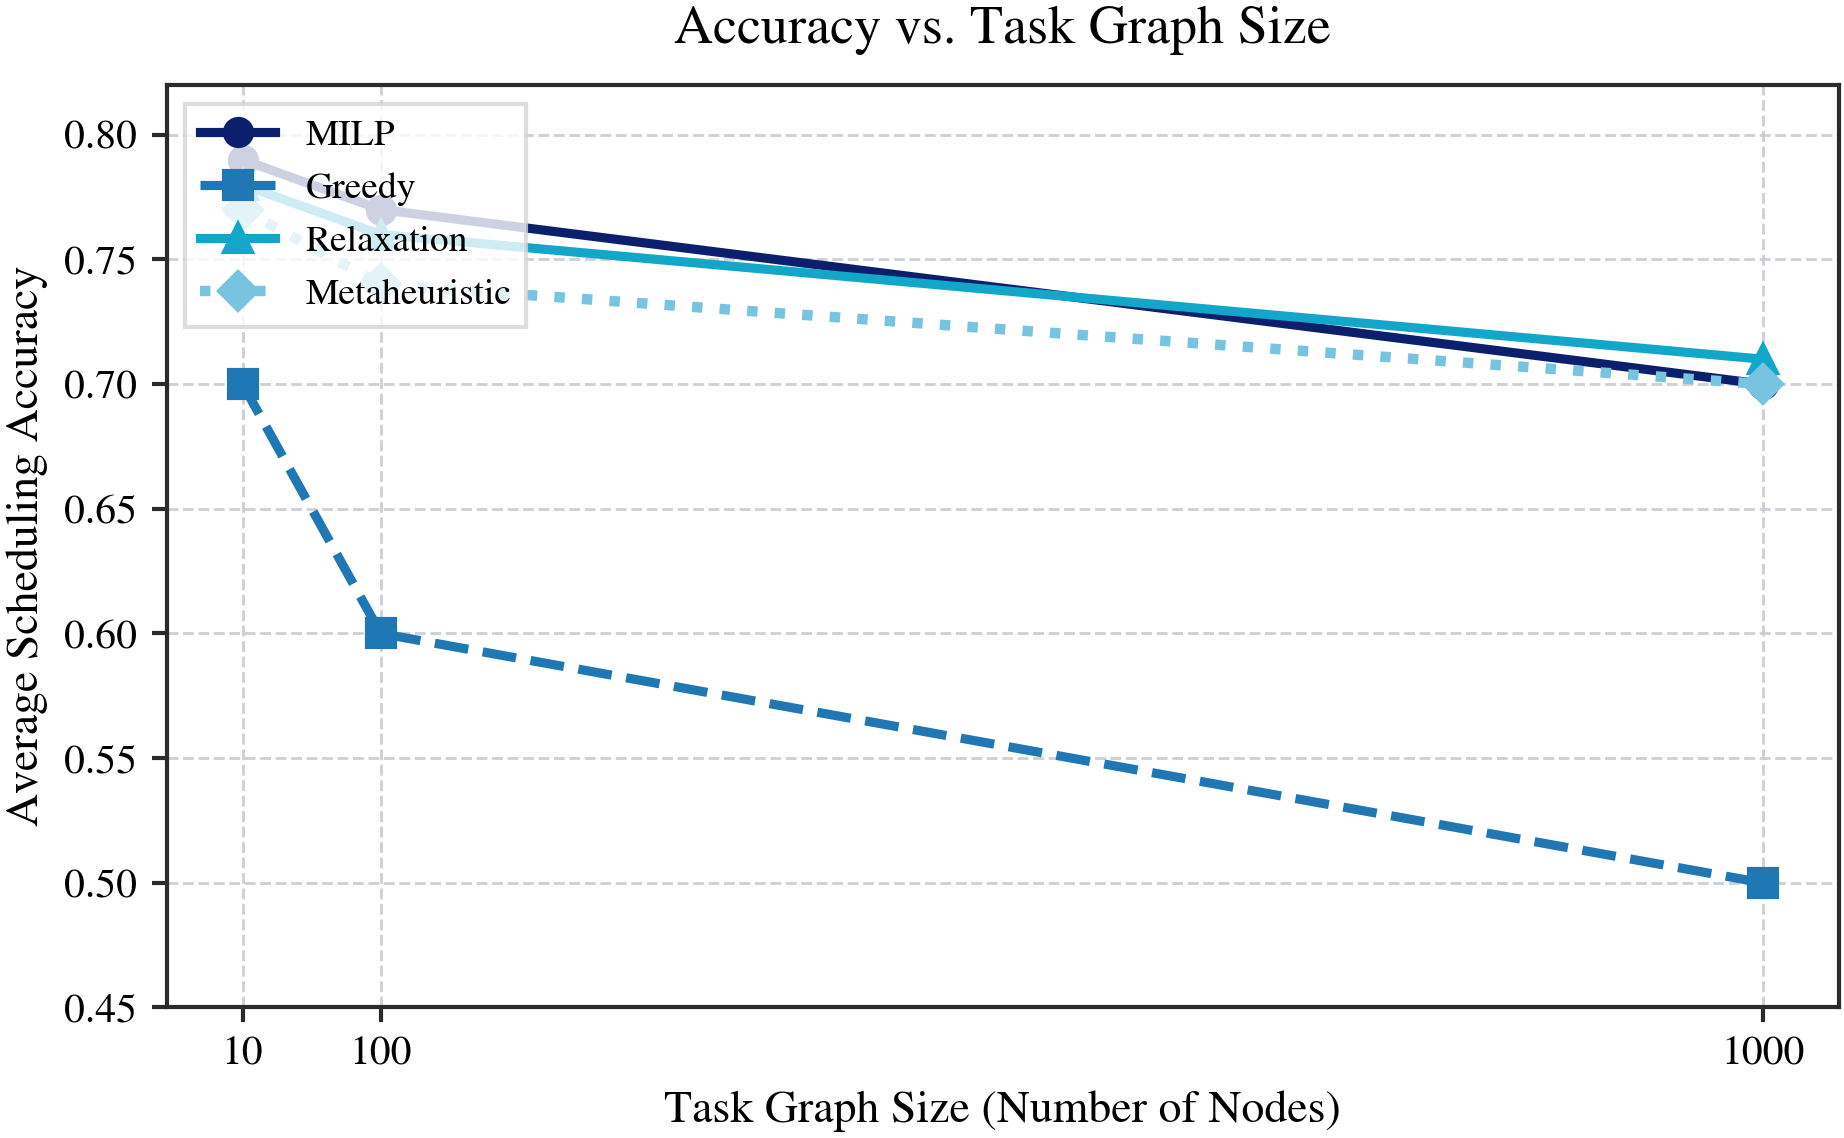
\includegraphics[width=0.95\linewidth]{Figures/perf_task_size_accuracy.png}
\caption{Reported average-accuracy score vs.\ DAG size. The MILP, randomized rounding, and GA remain clustered near 0.70 at 1000 tasks, while the greedy falls to about 0.50.}
\label{fig:tasksize}
\end{figure}

\subsection{Task Failures}

Fig.~\ref{fig:failure} shows accuracy as the per-task failure rate rises from 0\% to 50\%. Every method degrades---failures directly remove accuracy---but the ranking is stable: the MILP falls from about 1.0 to 0.75, randomized rounding and the GA track it down to about 0.71, and the greedy degrades fastest, ending near 0.60. The global methods lose less because they can reroute around failed or degraded placements while still pricing the data transfers involved; the greedy has no mechanism to rebalance once early commitments go wrong.

\begin{figure}[h!]
\centering
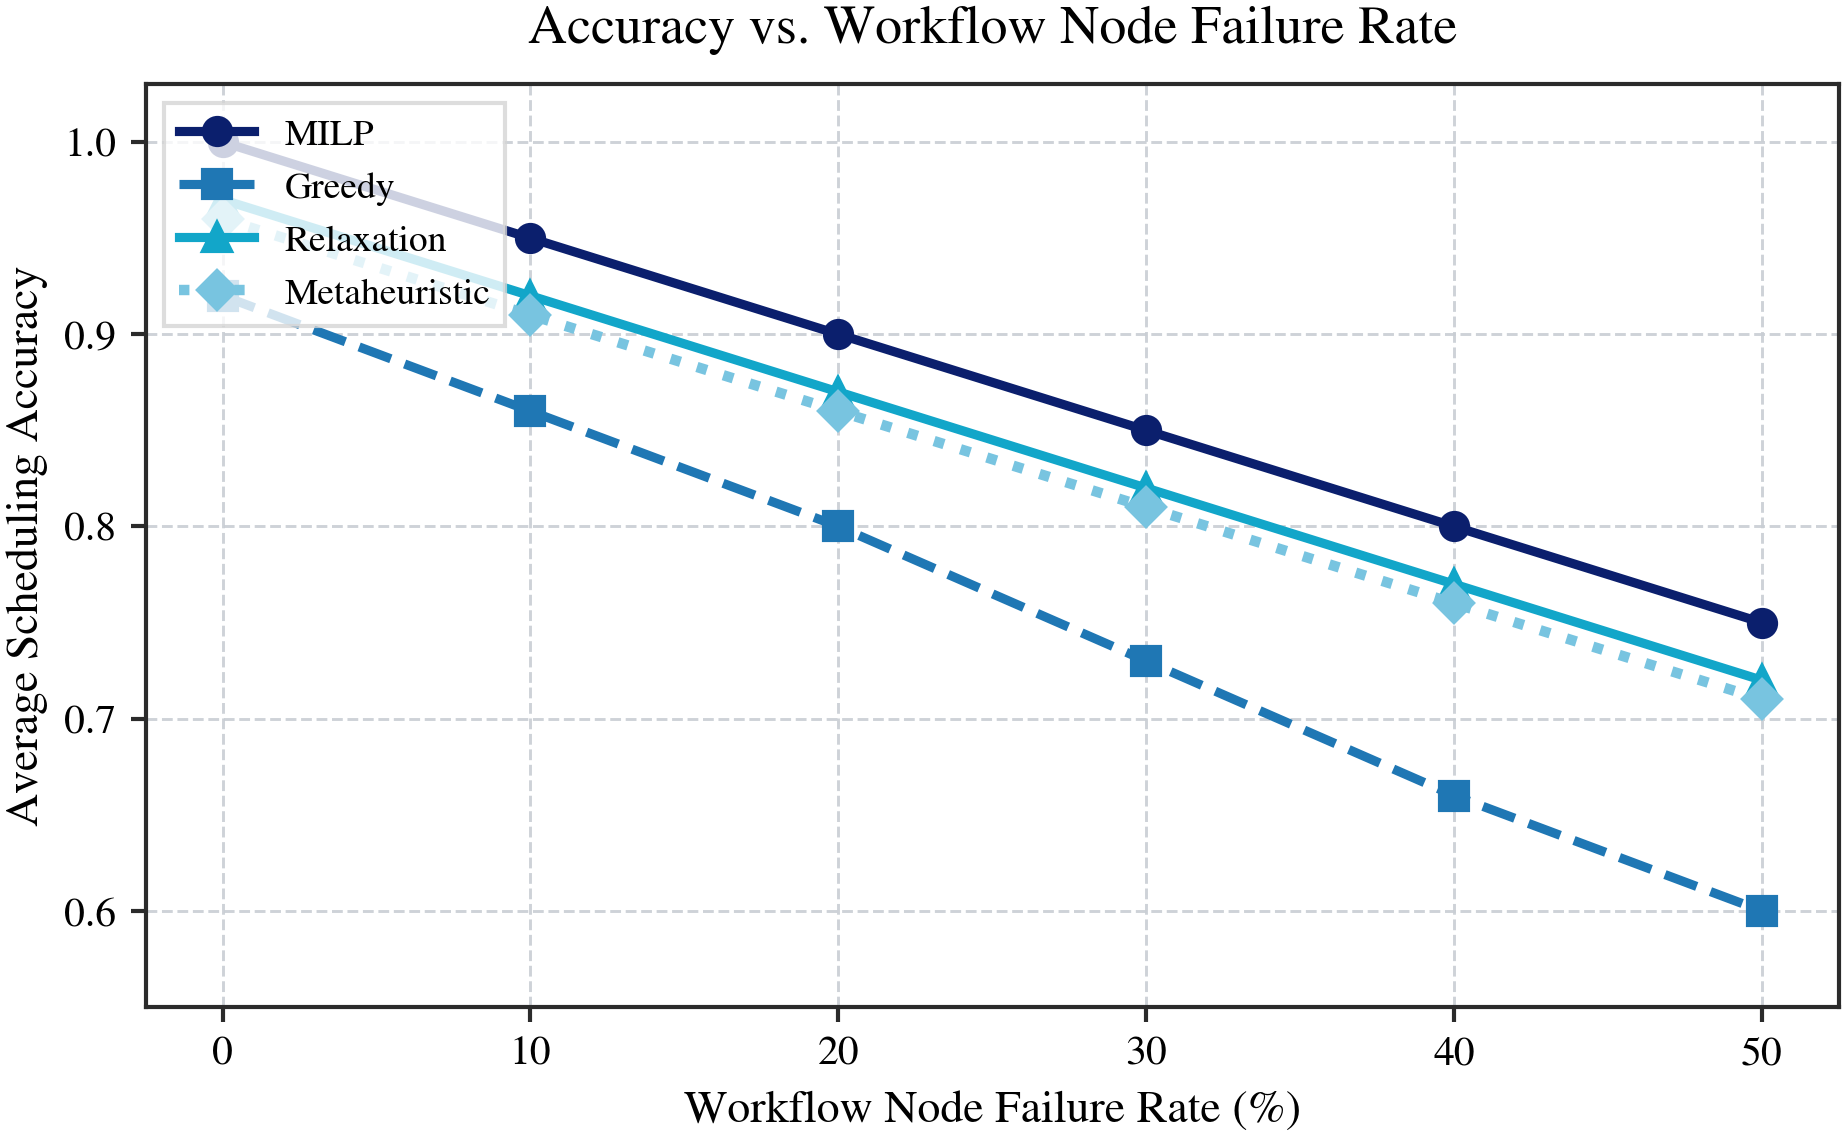
\includegraphics[width=0.95\linewidth]{Figures/perf_failure_accuracy.png}
\caption{Average scheduling accuracy vs.\ task failure rate. The MILP degrades most gracefully; the greedy loses the most.}
\label{fig:failure}
\end{figure}

\subsection{Discussion}

Three observations summarize the experiments. First, the gap between methods is largest exactly where the problem is hardest---tight deadlines and high failure rates---so the choice of scheduler matters most in the disaster regime that motivates the paper. Second, randomized rounding is the best practical default: it stays within a few points of the MILP in every experiment at a fraction of the solve time. Third, the GA is the most robust of the scalable methods at large sizes and high failure, while the greedy is useful mainly as a fast, transparent fallback.

\subsection{Positioning Within the Literature}

Section~\ref{sec:related} described why no off-the-shelf scheduler is a drop-in comparator: HEFT-style methods assume full execution, fog schedulers are compute-centric, and approximate-computing schedulers do not model inter-node data movement. Because the joint formulation is new, the fair comparisons are the ones reported here---the proposed methods against each other and against the fixed-slack and max-accuracy reference policies---and the MILP's role is to certify how much accuracy the scalable methods leave on the table. Adapting existing DAG schedulers to the present problem class is left to future work.

\section{Conclusion and Future Work}

This paper formulated data- and bandwidth-aware scheduling of approximate DAG workflows in federated fog systems as a mixed-integer linear program, and gave three scalable schedulers built on the same cost model. In simulation, the MILP sets the accuracy ceiling; randomized rounding consistently comes closest to it; the genetic algorithm is the most robust scalable method at large workflow sizes and high failure rates; and the bandwidth-aware greedy is fastest but loses the most accuracy where slack is tight.

Future work has three directions. \textbf{Online adaptation:} re-scheduling as workloads, links, and node availability change during an event. \textbf{Graph compression and partitioning:} simplifying large DAGs and placing subgraphs rather than single tasks to reduce both solve time and inter-node traffic. \textbf{Field deployment:} running the schedulers on a real federated fog testbed with space-sharing and isolation, so the model's assumptions can be validated against measured transfers and failures.

\section*{Acknowledgments}

We thank the anonymous reviewers for their valuable feedback. This research is supported by the National Science Foundation (NSF).

\appendix
\section{Correctness and Linearization}
\label{app:proofs}

This appendix shows that the formulation of Section~\ref{sec:milp} means what it should, and how to write it for a standard MILP solver. A solution is \emph{feasible} if every task is placed on exactly one permitted node, at most one $l_{ia}$ per task is non-zero, and all tasks complete by $t_{\max}$.

\begin{lemma}
\label{lem:elig}
If $P_{ia}=0$ then $e_{ia}=0$.
\end{lemma}
\begin{proof}
Immediate from \eqref{eq:elig} and $e_{ia}\in\{0,1\}$.
\end{proof}

\begin{lemma}
\label{lem:one}
Every task is assigned to exactly one node.
\end{lemma}
\begin{proof}
By \eqref{eq:one}, $\sum_a e_{ia}=1$ with $e_{ia}$ binary.
\end{proof}

\begin{lemma}
\label{lem:frac}
For each task, at most one $l_{ia}$ is non-zero, and $l_{ia}>0$ implies $e_{ia}=1$.
\end{lemma}
\begin{proof}
$l_{ia}>0\Rightarrow e_{ia}\ge l_{ia}>0\Rightarrow e_{ia}=1$ by \eqref{eq:frac}, and Lemma~\ref{lem:one} leaves no other node with $e_{ia}=1$.
\end{proof}

\begin{lemma}
\label{lem:timing}
$M_{ia}$ is the earliest time $T_i$ can start on $f_a$, and $y_i$ is the completion time of $T_i$ on the node it is assigned to.
\end{lemma}
\begin{proof}
Induction on the distance of $T_i$ from a source. A source task has $\mathrm{in}_i=\varnothing$, so $M_{ia}=0$ by \eqref{eq:startsrc} and $y_i=\sum_a e_{ia}(M_{ia}+t_{ia}l_{ia})=t_{ia^{\star}}l_{ia^{\star}}$ on its assigned node $f_{a^{\star}}$ by Lemma~\ref{lem:one}. For the step, suppose the claim holds for every task whose distance from a source is less than $k$, and let $T_i$ have distance $k$. Every $T_j\in\mathrm{in}_i$ completes at $y_j$ on its assigned node $f_{b^{\star}}$; the data then needs $c_{ji}^{b^{\star}a}=\sum_b e_{jb}c_{ji}^{ba}$ to reach $f_a$, so $T_i$ cannot start on $f_a$ before $y_j+\sum_b e_{jb}c_{ji}^{ba}$. Taking the maximum over $j\in\mathrm{in}_i$ gives exactly \eqref{eq:start}, and \eqref{eq:compl} gives $y_i$.
\end{proof}

\begin{lemma}
\label{lem:deadline}
All tasks complete by $t_{\max}$.
\end{lemma}
\begin{proof}
By Lemma~\ref{lem:timing} and \eqref{eq:deadline}.
\end{proof}

\begin{theorem}
Any optimal solution of \eqref{eq:obj}--\eqref{eq:bin} is feasible and maximizes the total achieved accuracy $\sum_i A_i\sum_a l_{ia}$.
\end{theorem}
\begin{proof}
Lemmas~\ref{lem:elig}--\ref{lem:deadline} establish feasibility. Optimality of the accuracy total is the objective \eqref{eq:obj} itself.
\end{proof}

For a solver, two constraints need rewriting. First, \eqref{eq:compl} contains the products $e_{ia}M_{ia}$. Introduce $z_{ia}=e_{ia}M_{ia}$ and replace \eqref{eq:compl} with
\begin{equation}
 y_i=\sum_{f_a\in F} z_{ia}+\sum_{f_a\in F} t_{ia}l_{ia},
\label{eq:compllin}
\end{equation}
together with the standard big-$M$ constraints
\begin{align}
 z_{ia} &\le t_{\max}\, e_{ia},\\
 z_{ia} &\le M_{ia},\\
 z_{ia} &\ge M_{ia}-(1-e_{ia})\,t_{\max},
\end{align}
which force $z_{ia}=M_{ia}$ when $e_{ia}=1$ and $z_{ia}=0$ otherwise. Second, \eqref{eq:start} is already in solver-friendly form: since $c_{ji}^{ba}$ are constants, each inequality is linear once written out per predecessor. The equalities \eqref{eq:startsrc} for source tasks are imposed directly.

\begin{theorem}
The linearized formulation has the same feasible placements and the same optimal accuracy as \eqref{eq:obj}--\eqref{eq:bin}.
\end{theorem}
\begin{proof}
For each $i$, exactly one $a$ has $e_{ia}=1$ (Lemma~\ref{lem:one}); on that node the $z$-constraints give $z_{ia}=M_{ia}$, and on all others $z_{ia}=0$, so \eqref{eq:compllin} reproduces \eqref{eq:compl} term by term. All other constraints are unchanged.
\end{proof}

\bibliographystyle{ieeetr}
\balance
\bibliography{cas-refs}

\end{document}
